%% The first command in your LaTeX source must be the \documentclass command.
%%
%% Options:
%% twocolumn : Two column layout.
%% hf: enable header and footer.
\documentclass[
% twocolumn,
% hf,
]{ceurart}

%%
%% One can fix some overfulls
\sloppy

%%
%% Minted listings support 
%% Need pygment <http://pygments.org/> <http://pypi.python.org/pypi/Pygments>
\usepackage{listings}
\usepackage{xcolor}
\usepackage{cleveref}
\usepackage{amsthm}

\usepackage[export]{adjustbox}

%% auto break lines
\lstset{language=Python, breaklines=true}

\newtheorem{example}{Example}
\newtheorem{definition}{Definition}
\newtheorem*{theorem*}{Theorem}

\newcommand{\red}[1]{\color{red}#1}

%% end of the preamble, start of the body of the document source.
\begin{document}


%%
%% Rights management information.
%% CC-BY is default license.
\copyrightyear{2023}
\copyrightclause{Copyright for this paper by its authors.
  Use permitted under Creative Commons License Attribution 4.0
  International (CC BY 4.0).}

%%
%% This command is for the conference information
\conference{BEWARE23: Workshop on Bias, Risk, Explainability and the role of Logic and Logic Programming, 6--9 November 2023, Rome, Italy}

%%
%% The "title" command
\title{BRIOxAlkemy: A Bias detecting tool}

\tnotemark[1]
\tnotetext[1]{%
% You can use this document as the template for preparing your publication. We recommend using the latest version of the ceurart style.
Work funded by the PRIN project n.2020SSKZ7R BRIO (Bias, Risk and Opacity in AI).}

%%
%% The "author" command and its associated commands are used to define
%% the authors and their affiliations.

\author[1]{Greta Coraglia}[
email=greta.coraglia@unimi.it
]
\author[3]{Fabio Aurelio D'Asaro}[
email=fabio.dasaro@univr.it
]
\author[1]{Francesco A. Genco}[%
email=francesco.genco@unimi.it
]
\author[2]{Davide Giannuzzi}[
  email=davide.giannuzzi@alkemy.com
  ]
\author[2]{Davide Posillipo}[
email=davide.posillipo@alkemy.com
]
\author[1]{Giuseppe Primiero}[
email=giuseppe.primiero@unimi.it
]
\author[2]{Christian Quaggio}[
email=christian.quaggio@alkemy.com
]

%\author[1,2]{Dmitry S. Kulyabov}[%
%orcid=0000-0002-0877-7063,
%email=kulyabov-ds@rudn.ru,
%url=https://yamadharma.github.io/,
%]
%\cormark[1]
%\fnmark[1]
%\address[1]{Peoples' Friendship University of Russia (RUDN University),
%  6 Miklukho-Maklaya St, Moscow, 117198, Russian Federation}
%\address[2]{Joint Institute for Nuclear Research,
%  6 Joliot-Curie, Dubna, Moscow region, 141980, Russian Federation}

%\fnmark[1]
\address[1]{LUCI Group, Department of Philosophy, University of Milan, via Festa del Perdono 7, 20122 Milan, Italy}
\address[2]{Alkemy, Deep Learning \& Big Data Department}
\address[3]{Ethos Group, Department of Human Sciences, University of Verona, Lungadige Porta Vittoria 17, 37129 Verona, Italy}

%\author[4]{Manfred Jeusfeld}[%
%orcid=0000-0002-9421-8566,
%email=Manfred.Jeusfeld@acm.org,
%url=http://conceptbase.sourceforge.net/mjf/,
%]
%\fnmark[1]
%\address[4]{University of Skövde, Högskolevägen 1, 541 28 Skövde, Sweden}

%% Footnotes
\cortext[1]{Corresponding author.}
%\fntext[1]{These authors contributed equally.}

%%
%% The abstract is a short summary of the work to be presented in the
%% article.
\begin{abstract}
We present a tool for the detection of biased behaviours in AI systems. Using a specific probability-based algorithm,
%typed $\lambda$-calculus, 
we provide the means to compare the action of the user's algorithm of choice on a specific feature that they deem ``sensible'' with respect to fixed classes and to a known optimal behaviour.
\end{abstract}

%%
%% Keywords. The author(s) should pick words that accurately describe
%% the work being presented. Separate the keywords with commas.
\begin{keywords}
Bias, Machine Learning, AI
\end{keywords}

%%
%% This command processes the author and affiliation and title
%% information and builds the first part of the formatted document.
\maketitle

\section{Introduction}
\label{sec:intro}


The project BRIO aims at developing formal and conceptual frameworks for the analysis of AI systems and for the advancement of the technical and philosophical understanding of the notions of Bias, Risk and Opacity in AI, with the ultimate objective of generally contributing to the development of trustworthy AI.\footnote{\url{sites.unimi.it/brio}} 

The aim of the collaboration between BRIO and Alkemy is to produce software applications for the analysis of bias, risk and opacity with regard to AI technologies which often rely on non-deterministic computations and  are often opaque in nature. One of the most challenging aspects of modern AI systems, indeed, is that they do not guarantee specification correctness, and they are not transparent, in the sense that a general formal description of their behaviour might not be available.

We present a first tool developed within the BRIOxAlkemy collaboration for the detection and analysis of biased behaviours in AI systems. The tool is aimed at developers and data scientists that wish to test their algorithms relying on probabilistic and learning mechanisms in order to detect misbehaviours related to biases and collect data about them. The ultimate goal is to provide them with useful insights and data for the improvement of the AI systems with respect to bias.

The system presented is based on the theoretical, foundational works presented in \cite{dap21}, \cite{dagp22}, and \cite{gp23}, and in this paper we discuss the formal ideas behind its development (Section \ref{sec:theory}), the technical details of its implementation  (\Cref{sec:implementation}), the data obtained from a case study that validates the usefulness of the software (\Cref{sec:validation}), and the projected further developments aimed at integrating the presented software in a more general tool for the analysis of AI systems (\Cref{sec:conclusions}).

\section{Theory}\label{sec:theory}

Our tool takes as input an AI model's output and a set of user's selected parameter settings: the former is encoded as a set of datapoints with their associated features, the latter include the designation of a sensitive feature. The output is an evaluation of the possibility that the AI model under consideration is biased with respect to the features designated as sensitive by the user. The system closely guides the user in the process of setting the parameters and provides it with detailed explanations, remaining customisable with respect to the mathematical details of the analysis. The choices left to the user are those that actually make a conceptual difference in the outcome of the analysis and this difference is explained to the user during the setting of these parameters.

The analyses conducted by our system are of two kinds: 

\begin{enumerate}
	\item comparison between the behaviour of the AI system and a target desirable behaviour (expressed as ``freq-vs-ref'' in the implementation), and
	
	\item comparison between the behaviour of the AI system with respect to a sensitive class $c_1\in F$ and the behaviour of the AI system with respect to another sensitive class $c_2\in F$ related to the same sensitive feature $F$ (expressed as ``freq-vs-freq'' in the implementation).
\end{enumerate}

Whenever the second behaviour alerts of a possibly biased behaviour, a subsequent check follow on some (or all) of the subclasses of the considered sensitive classes. This second check is meant to tell us if the bias encountered at the level of the classes can be explained away by other features of the individuals in the sensitive classes considered that are not related to the sensitive feature at hand.

Before we delve into the technical details, let us give a little example: 

\begin{example}
Consider a database containing details of individuals, with their age, gender, and level of education. Consider an algorithm which tries to predict whether each of them is likely to default on credit. We wish to check if age is a sensitive factor in such prediction. We feed the tool our dataset, the output of the run of the predictive algorithm, and mark the feature of age as sensitive. The program allows us to compare either how the behaviour of the algorithm with respect to age differs from an ``optimal'' behaviour (in this case, we might consider optimal the case where each age group equally succeeds), or how different age groups perform with respect to one another.
\end{example}
 
\subsection{Divergences}
The comparisons above are computed on probability distributions, each taken to express the behaviour of a stochastic system. In order to compute the difference between the behaviour of the AI system under investigation -- denoted by the probability distribution $Q$ -- and a fixed behaviour $P$ (either the optimal behaviour, when available, or the behaviour with respect to a different class) various means of comparison might be considered. Depending on the analysis one wishes to conduct, one or more divergences or distances are made available in the tool. Notice that all divergences and distances are made to take values in $[0,1]$ in order to be compared with the threshold described in \Cref{threshold}.


\paragraph{Kullback-Leibler divergence}
When we wish to compare how the system behaves with respect to an \textit{a priori} optimal behaviour $P$, we use the Kullback–Leibler divergence $D_{\mathrm{KL}}$:

\[D_{\mathrm{KL}}(P\parallel Q)= \sum _{x\in X} P(x)\cdot \log_2 \Big( \frac{P(x)}{Q(x)}\Big)\,.\]

It was first introduced in \cite{dkl} in the context of information theory, and it intuitively indicates the difference, in probabilistic terms, between the input-output behaviour of the AI system at hand and a reference probability distribution. It sums up all the differences computed for each possible output of the AI system weighted by the actual probability of correctly obtaining that output.

Notice that this is not symmetric and takes values in $[0,+\infty]$: the asymmetry accounts for the fact that the behaviour we are monitoring is, in fact, non symmetric -- as $P$ is a theoretical distribution that we know, or consider to be, optimal, while $Q$ is our observed one -- while to make it fit the unit interval we adjust the divergence as follows.

\[D'_{\mathrm{KL}}(P\parallel Q)=1-\exp (- D_{\mathrm{KL}}(P\parallel Q))\]

\paragraph{Jensen-Shannon divergence}
When we wish to compare classes, instead, a certain symmetry is required. First, we consider the Jensen-Shannon divergence 
\[D_{\mathrm{JS}}(P\parallel Q)=\frac{D_{\mathrm{KL}}(P\parallel M)+D_{\mathrm{KL}}(Q\parallel M)}{2},\]
with $M=(P+Q)/2$. This was introduced in \cite{lin_divergence} as a well-behaved symmetrization of Kullback-Leibler. It takes values in $[0,1]$.

\paragraph{Total variation distance}
Another choice for comparing classes is provided by the total variation distance of $P$ and $Q$, meaning
\[D_{\mathrm{TV}}(P, Q)= \sup _{x\in X} \vert P(x) - Q(x)\vert,\]
which computes the largest difference between the probability of obtaining an output $o$ given in input individuals of distinct sensitive classes $c_1\in F$ and $c_2\in F$.\footnote{We write the argument $(P,Q)$ instead of $P\parallel Q$ to remark that this is in fact a distance, and not a divergence.}  It, too, takes values in $[0,1]$. %{\color{red} Since the value of $D_{\mathrm{TV}}$ is smaller than the value of $D_{\mathrm{JS}}$, it should only be used for toutine checks.}

%In order to normalise the values of the different divergences that we use in the system and be able to select common, reasonable thresholds for all of them, we project the values of $D_{\mathrm{KL}}$ and $D^{\mathrm{Sym}}_{\mathrm{KL}}$ onto the interval $[0,1]$. The divergences $D_{\mathrm{KL}}(P\parallel Q)$ and $D^{\mathrm{Sym}}_{\mathrm{KL}}(P\parallel Q)$ are replaced, respectively, by
%
%\[
%1-\frac{1}{D_{\mathrm{KL}}(P\parallel Q)} \quad\text{and}\quad 1-\frac{1}{D^{\mathrm{Sym}}_{\mathrm{KL}}(P\parallel Q)}\;.
%\]

%%NEW VERSION (?):
%In order to normalise the values of the different divergences that we use in the system and be able to select common, reasonable thresholds for all of them, we project the values of $D_{\mathrm{KL}}$ onto the interval $[0,1]$. The divergence $D_{\mathrm{KL}}(P\parallel Q)$ is thus replaced by
%
%\[1-\exp (- D_{\mathrm{KL}}(P\parallel Q))\]where the $\exp(x)$ function is defined as $e^x$. 

The theory provides a perhaps clearer description of total variation, and relates it with Jensen-Shannon as follows.

\begin{theorem*}[{\cite[Prop. 4.2]{levin2017markov}},{\cite[Thm. 3]{lin_divergence}}]
Let $P$ and $Q$ probability distributions over $X$. Then we have the following:
\begin{enumerate}
\item $D_{\mathrm{TV}}(P,Q)=\frac{1}{2}\sum_{x\in X}\vert P(x)-Q(x)\vert$;
\vspace{0.2cm}
\item $D_{\mathrm{JS}}(P\parallel Q)\leq D_\mathrm{TV}(P,Q)$.
\vspace{0.2cm}
\end{enumerate}
\end{theorem*}

This suggests that Jensen-Shannon is less sensitive to differences in the comparing sets, and can therefore be used for preliminary analyses.

\subsection{How to handle sensitive features corresponding to more than two classes}\label{subsec:aggregation}
Since the divergences the system uses are binary functions, it is not obvious how to handle the case in which the sensitive feature we are considering partitions the domain in three or more classes. It is, indeed, easy to compute the divergence for pairs of classes, but we also need, in this case, a sensible way of aggregating the obtained results in order to obtain one value describing well how the AI model behaves with respect to the sensitive feature under consideration. It turns out that there are several ways of doing this and each of them tells us something of value if we wish to reach a meaningful conclusion about the AI model.

Suppose that we are studying the behaviour of the model with respect to the feature $F=\{c_1, \ldots , c_n\}$ which induces a partition of our domain of individuals into the classes $c_1, \ldots , c_n$. The first step is the pairwise calculation of the divergences with respect to the different classes induced by $F$. Hence, for each pair $(c_i\parallel c_j)$ such that $c_i, c_j\in F$, we compute $D(c_i\parallel c_j) $ where $D$ is the  preselected divergence and consider the set $\{D(c_i\parallel c_j) : c_i,c_j\in F\ \&\ i\neq j\}$. For instance, if we are considering age as our feature  $F$ and we partition our domain into three age groups, we might have
\[F=\{over\_50\_yo, between\_40\_and\_50\_yo, below\_40\_yo\}\]
We can then use the following ways of aggregating the obtained values.

\paragraph{Maximal divergence}

$$\max (\{D(c_i\parallel c_j): c_i,c_j\in C\ \&\ i\neq j\})$$
Maximal divergence corresponds to the worst case scenario with respect to the bias of our AI system. This measure indicates how much the AI system favours the most favoured class with respect to the least favoured class related to our sensitive feature.

\paragraph{Minimal divergence}
$$\min (\{D(c_i\parallel c_j): c_i,c_j\in C\ \&\ i\neq j\})$$
Minimal divergence, on the other hand, corresponds to the best case scenario.  This measure indicates the minimal bias expressed by our AI system with respect to the sensitive feature. If this measure is $0$, we do not know much, but if it is much above our threshold, then we know that the AI system under analyis expresses strong biases with respect to all classes related to the sensitive feature.


\paragraph{Average of the divergences}
$$\sum_{c_i,c_j\in C} D(c_i\parallel c_j)/\binom{\mid C\mid}{2}$$
i.e. the sum of the divergences between the two elements of each pair $c_i,c_j\in C$ divided by the total number $\binom{\mid C\mid}{2}$ of these pairs. This measure indicates the average bias expressed by the AI system. Unlike the previous measures, this one meaningfully combines information about the behaviour of the system with respect to all classes related to the sensitive feature.  What this measure still does not tell us, though, is the variability of the behaviour of the system in terms of bias. The same average, indeed, could be due to a few very biased behaviours or to many mildly biased behaviours.


\paragraph{Standard deviation of the divergences}
\[\sqrt{ (\sum_{c_i,c_j\in C} (D(c_i\parallel c_j)-\mu)^2 / \binom{\mid C\mid}{2}  )}\] where  $\mu = \sum_{c_i,c_j\in C} D(c_i\parallel c_j)/\binom{\mid C\mid}{2}$. That is, the square root of the average of the squares of the divergences between each value $D(c_i\parallel c_j)$ and the average value of $D(c_i\parallel c_j)$ for each pair $c_i,c_j$. In other terms,  we calculate the average of the divergences, then the difference of each divergence with respect to their average, then we square this differences and calculate their average. Finally, we compute the square root of this average.
This measure indicates the variability of the bias expressed by the AI system we are inspecting. That is, how much difference there is between the cases in which the system is behaving in a very biased way and the cases in which the system is behaving in a mildly biased way. This information complements the information we can gather by computing the previous measure.

\subsection{Parametrisation of the threshold for the divergence}\label{threshold}

Whenever the system computes a divergence between the results of the model and a reference distribution or the results of the model for distinct classes, a threshold is employed to check whether the divergence is significant -- in which case it should be treated as a possible violation of our fairness criteria -- or negligible -- in which case should be simply ignored. Obviously, fixing this threshold once and for all would give a rather inflexible system. For instance, setting the threshold to $1/100$ might be reasonable if we are considering the results of the model on a set of $100$ individuals, but it is clearly too strict if our domain only contains $40$ individuals. In the latter case, even a difference only concerning one individual would constitute a mistake much greater than the one admitted by the threshold. This is why we parametrise the threshold on the basis of several factors. 

First, the user has to decide how much rigour is required when analysing the behaviour of the model with respect to the feature indicated as sensitive for the present analysis. Two settings are possible: 

\begin{itemize}
\item $\mathtt{high}$: it implies that the considered feature is very sensitive and that the system should be extra attentive about the behaviour of the model in relation to it;
\item $\mathtt{low}$: it implies that differences in the behaviour of the model with respect to the considered feature are significant only if they are particularly strong or extreme. This setting distinguishes between a thorough and rigorous investigation and a simple routine check, one might say.
\end{itemize}



The second factor considered in computing the threshold is the number of classes related to the sensitive feature under consideration. We  call this the {\it granularity} of the predicates related to the sensitive feature, and it indicates how specific the predicates determining the studied classes are. Specific predicates describe in more detail the objects of our domain and determine more specific classes. When the classes that we are considering are very specific, the divergence generated by the bias of the model can be spread over several different classes. Hence, we need to be more attentive about the small divergences that appear locally -- that is, when we check pairs of these classes. The threshold should thus be stricter.


Finally, each time we compute a divergence relative to two classes, we scale the threshold with respect to the cardinality of the two classes. Large classes mean a stricter threshold. This is a rather obvious choice related to the fact that statistical data related to a large number of individuals tend to be more precise and fine grained. We already gave an example of this few lines ago.

Technically, the threshold is always between $0.05$ and $0.005$, the setting $\mathtt{high}$ restricts this range to the interval $[0.005,0.0275]$ and the setting $\mathtt{low}$ to the interval $[0.0275,0.05]$. The number $n_C$ of classes related to the sensitive feature and the number $n_D$ of individuals in our local domain (that is, the cardinality of the union of the two classes with respect to which we are computing the divergence) are used to decrease the threshold (in other words, to make it stricter) proportionally with respect to the interval selected. The greater the number $n_C$, the smaller the threshold, the greater the number $n_D$, again, the smaller the threshold. The threshold is then computed as
\[
\epsilon = (n_C \cdot n_D) \cdot m + (1-(n_C \cdot n_D)) \cdot M
\]
where $m$ is the lower limit of our interval and $M$ is its upper limit.

\section{Implementation}
\label{sec:implementation}

A first Minimum Viable Product (MVP) for the outlined bias detection tool has been implemented using the programming language Python (3.x) and can be found at the following URL: \url{https://github.com/DLBD-Department/BRIO_x_Alkemy}. We present in this Section the most relevant aspects of the implementation.

\subsection{Backend}
\label{subsec:backend}

In terms of software architecture, the tool leverages on Docker in order to reach full portability. Currently it uses a simple python:3.10 image sufficient for early developments. The tool is developed following the Object Oriented Programming (OOP) paradigm in order to make allow easy extension to the upcoming functionalities both for bias and opacity detection. In this section a few details about the implemented classes are provided. 

\paragraph{\texttt{BiasDetector} class}

This class contains the methods shared by both bias detection tasks described in Section \ref{sec:theory}, namely \texttt{freqs-vs-ref} and \texttt{freqs-vs-freqs}. In particular, this class contains the method \texttt{get\_frequencies\_list} which is used compute the distribution of the dataframe units with respect to the target feature (\texttt{target\_variable} in the code), the output of a predictive machine learning model, conditioned to the categories of the sensitive features (\texttt{root\_variable} in the code). 

\paragraph{\texttt{Freqs-vs-RefBiasDetector} class}
This class inherits from \texttt{BiasDetector} and implements the freqs-vs-ref analysis described in Section \ref{sec:theory}. The constructor of the class provides the option for the normalization of the KL divergence. The KL divergence calculation is implemented in the method \texttt{compute\_distance\_from\_reference}. Currently only the discrete version of KL is implemented. 

The method \texttt{compare\_root\_variable\_groups} computes the distance, in terms of normalized KL divergence, of the observed distribution of \texttt{target\_variable} conditioned to \texttt{root\_variable} with respect to a reference distribution that is passed as parameter.

The method \texttt{compare\_root\_variable\_conditioned\_groups} performs the same calculation described above but for each sub-group implied by the Cartesian product of the categories of \texttt{conditioning\_variables}, a list of available features present in dataframe and selected by the user. The computation is performed only if the sub-groups are composed of at least \texttt{min\_obs\_per\_group} observations, with a default of 30. 

\paragraph{\texttt{FreqVsFreqBiasDetector} class}
This class inherits from \texttt{BiasDetector} and implements the freqs-vs-freqs analysis described in Section \ref{sec:theory}. The constructor of the class provides the options for setting up the aggregation function for the multi-class case (see Section \ref{subsec:aggregation}), for the selection of the A1 parameter value for the parametric threshold (see Section \ref{threshold}) and for the distance definition to be used for the calculations. Currently only JS and TVD are supported. 

The method \texttt{compute\_distance\_between\_frequencies} computes the JS divergence or the TV distance as selected for the \texttt{observed\_distribution}, an array with the distribution of the \texttt{target\_variable} conditioned to \texttt{root\_variable}. The final value is provided using the selected aggregation function, relevant in case of multi-classes root variables. 

The method \texttt{compare\_root\_variable\_groups} computes the mutual distance, in terms of JS or TVD, of the categories of the observed distribution of \texttt{target\_variable} conditioned to \texttt{root\_variable}.

The method \texttt{compare\_root\_variable\_conditioned\_groups} performs the same calculation described above but for each sub-group implied by the Cartesian product of the categories of \texttt{conditioning\_variables}, with the same constraints as for the \texttt{Freqs-Vs-RefBiasDetector} class.

%that is a list of available features present in dataframe and selected by the user. The computation is performed only if the sub-groups are composed of at least \lstinline[columns=fixed]{min_obs_per_group} observations, with a default of 30.

\paragraph{Threshold calculator}
When the threshold is not provided by the user, the tool computes it using the \texttt{treshold\_calculator} function, which implements the algorithm described in Section \ref{threshold}.

\subsection{Frontend}

For the frontend implementation, the tool relies on Flask, a  framework for building web applications in Python. It provides great flexibility and modularity with the \textit{routing} mechanism, allowing the user to select which URL should trigger which python function. This makes it straightforward to create distinct endpoints for various parts of the application. Routes that respond to different HTTP methods (GET, POST, etc.) and render dynamic content can thus be easily created.

The user can investigate and analyse bias behaviour in a given AI system by accessing the \textit{Bias} section of the frontend. They have the possibility to upload either an already preprocessed dataframe, or a raw dataset together with a customised preprocessing pipeline, see Figure \ref{fig:bias_upload}.

\begin{figure}[h]
  \begin{center}
    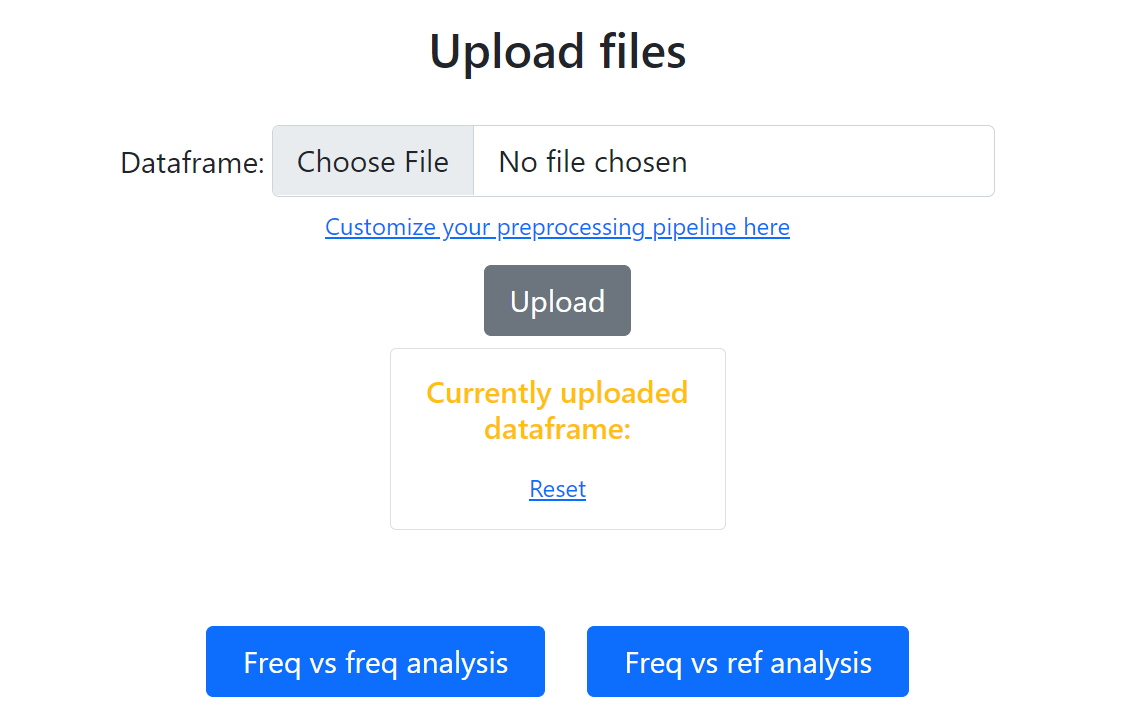
\includegraphics[width=0.8\textwidth]{frontend_bias_upload.png}
  \end{center}
  \caption{Upload options for the bias detection tool}
  \label{fig:bias_upload}
\end{figure}


Afterwards, the user can compare the behaviour of the AI system with an ideal behaviour (Frequence vs Frequence), or compare sensitive classes within the AI system itself (Frequence vs Reference), also shown in Figure \ref{fig:bias_upload}.

\subsubsection{FreqVsFreq and FreqVsRef}
To perform these analyses, a set of parameters have to be chosen. Firstly, the \textbf{distance}: the choice is between \textit{Total Variation Distance} and \textit{Jensen-Shannon Divergence} for \textbf{FreqVsFreq}, and \textit{Kullback-Leibler Divergence} is used for \textbf{FreqVsRef}. Then, the user has to select: 

\begin{itemize}
  \item the target feature;
  \item the sensitive feature;
  \item \textit{FreqVsFreq exclusive}: the aggregating function (only when the sensitive feature partitions the domain in three or more classes);
  \item the threshold (this can also be automatically computed, see Section \ref{threshold});
  \item additional conditioning features, which further split the domain into subclasses;
  \item \textit{FreqVsRef exclusive}: the reference distributions, which will depend on the target and the sensitive features. 
\end{itemize}

\subsubsection{Results}
Eventually, the tool shows the analysis results, providing insights about whether the AI system under investigations presents behaviour that might be interpreted as bias with respect to the sensitive feature. This is implemented in a boolean variable, which is \textbf{\textcolor{red}{False}} when bias is present and \textbf{\textcolor{green}{True}} otherwise, as it is shown in Figure \ref{fig:results}.

\begin{figure}[h]
  \begin{center}
    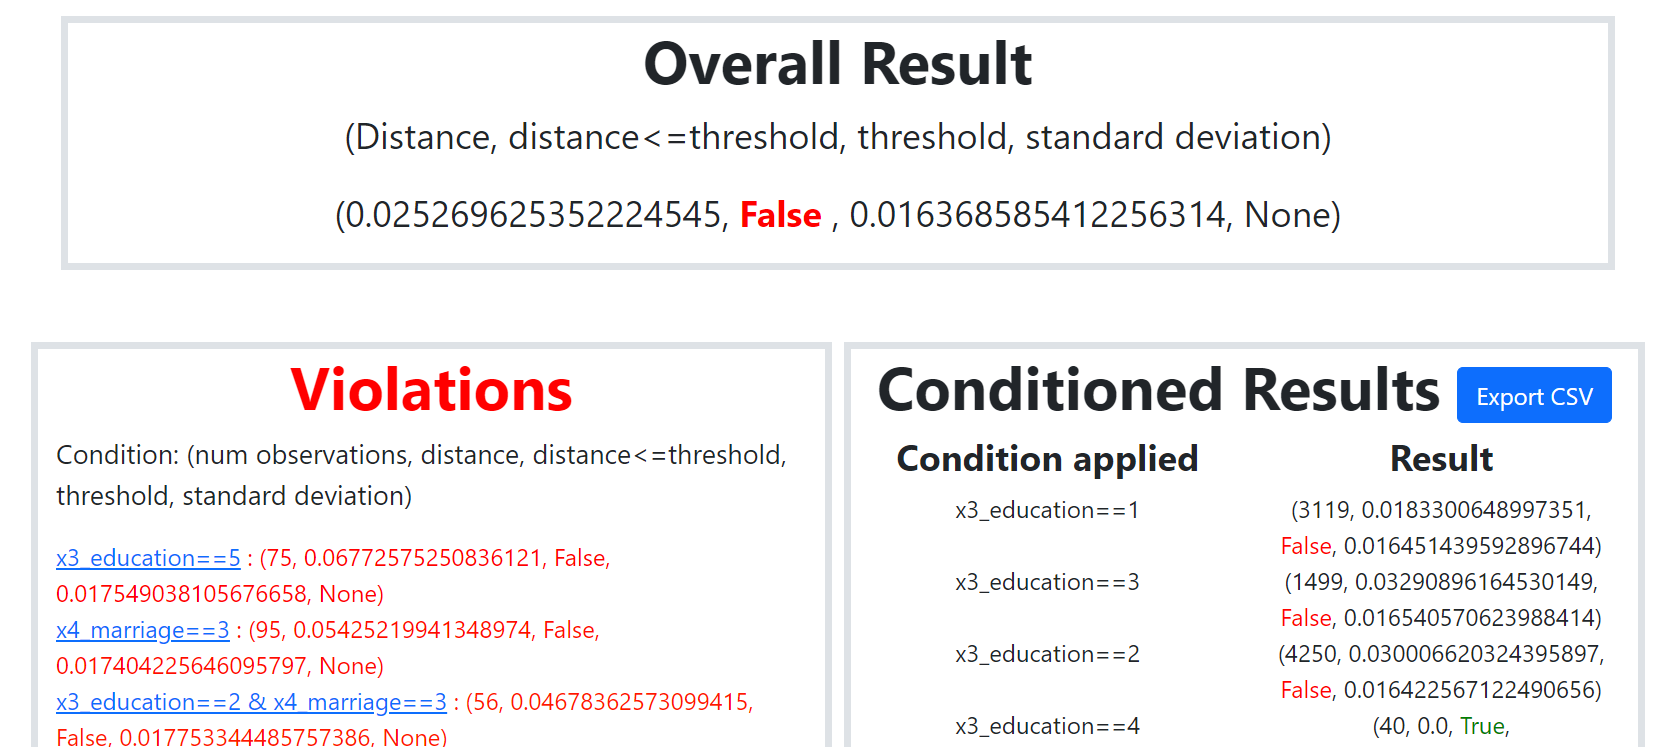
\includegraphics[width=0.8\textwidth]{frontend_results_page.png}
  \end{center}
  \caption{Results page displaying comprehensive results from all subclasses (top), subclass-specific violations (bottom left), subclass-specific results (bottom right)}
  \label{fig:results}
\end{figure}

If bias behavior is detected, additional information at the subclass level (if applicable) are also presented, ranked from most severe to less significant. Furthermore, results for each subclass are also displayed, with the possibility to export the data in a csv file for additional studies. 

\section{Validation}
\label{sec:validation}

A set of experiments were performed to understand the behavior of the proposed approach on real data, in particular for the freqs-vs-freqs analysis. To simulate a realistic bias detection scenario, payment data from a cash and credit card issuer in Taiwan published in \cite{YEH20092473} were used. The targets were credit card holders of the bank. 

As first step, three machine learning models were trained to predict the default probability, using all the available features:

\begin{itemize}
  \item ``strong'' model: a Random Forest with 200 trees and max depth equals to 12;
  \item ``weak'' model: a Random Forest with 10 trees and max depth equals to 37;
  \item ``lame'' model: a Classification Tree with max depth equals to 2.
\end{itemize}

Training and performance details of the three models are available on the GitHub repository \url{https://github.com/DLBD-Department/BRIO_x_Alkemy/notebooks}. The three models show different performance in terms of accuracy and errors distribution: the aim is to verify if and how our bias detection tool deals with such different models performances. 

\subsubsection{Experiment 1: freqs-vs-freqs, TVD, A1=low, root-variable=x2-sex}

\begin{figure}[h!]
  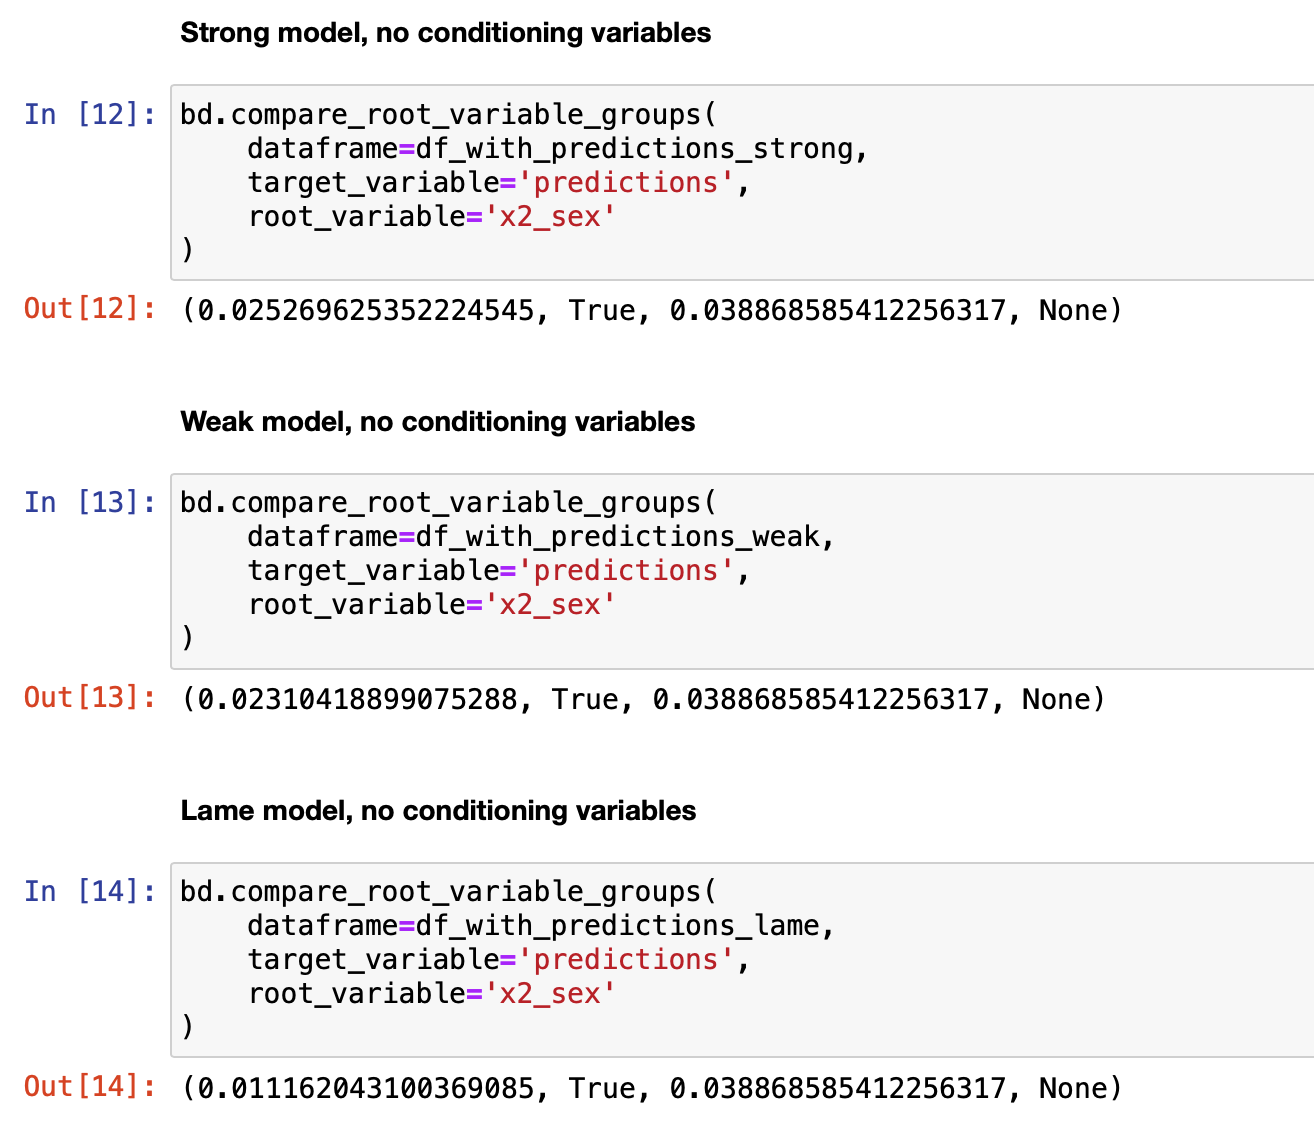
\includegraphics[width=.8\linewidth, left]{exp1.png}
  \caption{Experiment 1 results.}
  \label{fig:exp1}
\end{figure}
Figure \ref{fig:exp1} shows the results of the first experiment. Using TVD and the parametric threshold, no bias is detected for the three models predictions (see output \texttt{True} on all three models), but the different distance magnitude obtained for the ``lame'' model is noticeable ($0,0278$, rounding off at the fourth decimal digit), and considerably smaller than those of the other two models (respectively $0,0138$ for the strong model and $0,0158$ for the weak model). A simpler, more erroneous model is unable to produce a strongly skewed predictions distribution and so it tends to produce ``less bias''. The ``strong'' model obtains the largest distance, suggesting that the more powerful a model is, the more likely it is to exploit predictive signals, producing more skewed predictions distributions. 

\subsubsection{Experiment 2: freqs-vs-freqs, TVD, A1=low, root-variable=x3-education}

\begin{figure}[h!]
  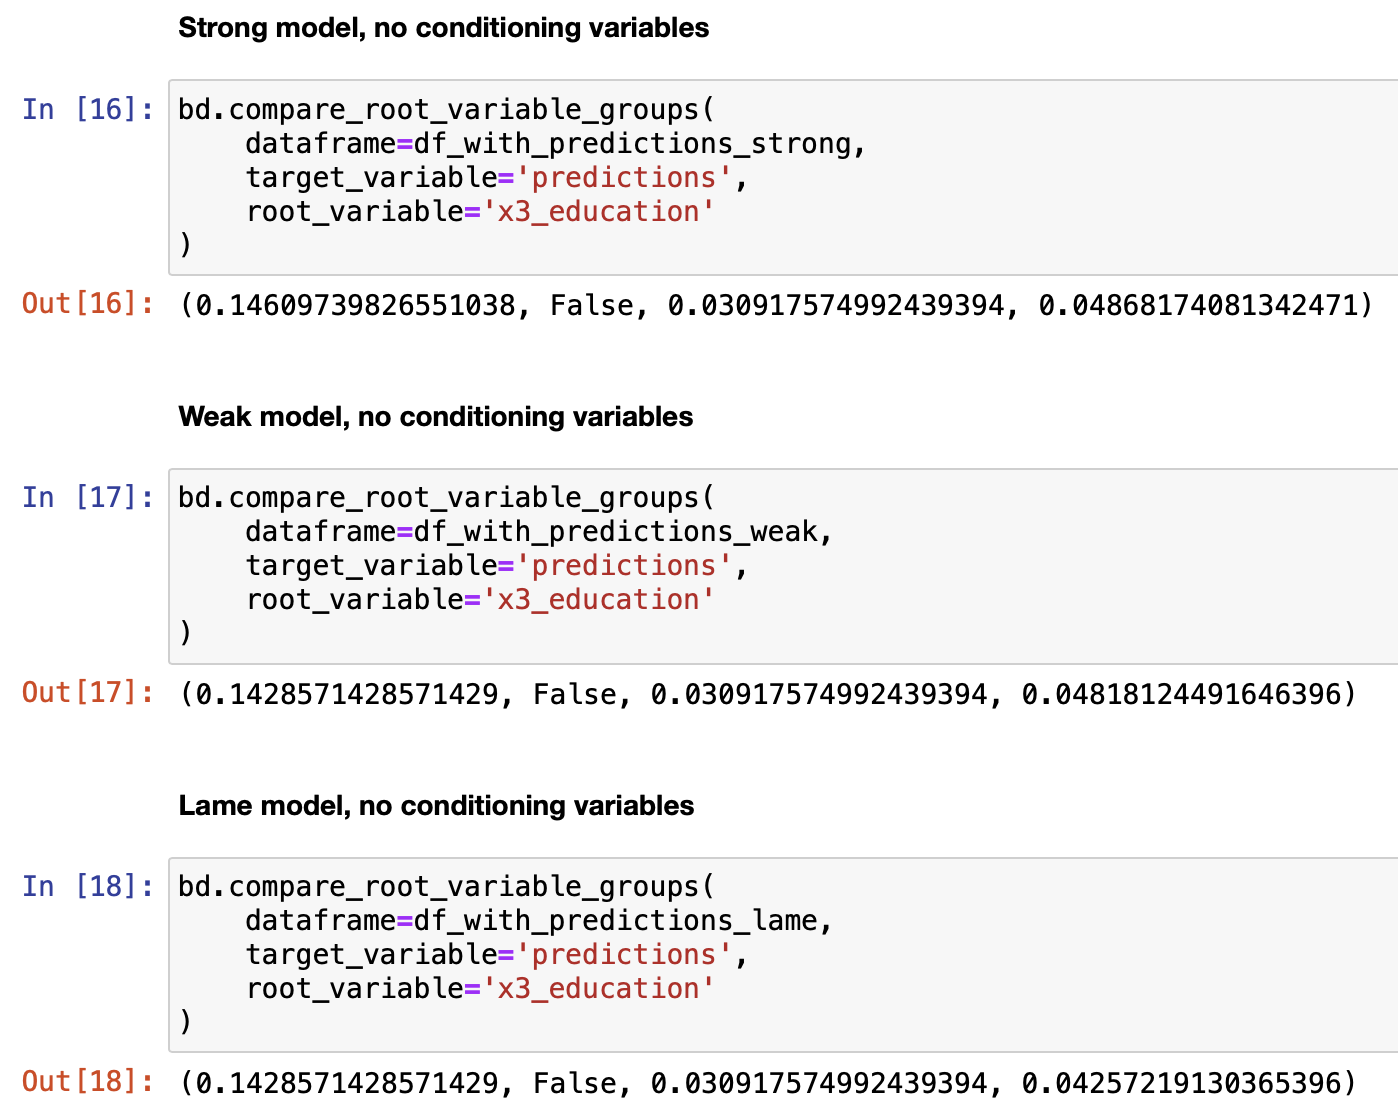
\includegraphics[width=.8\linewidth, left]{exp2.png}
  \caption{Experiment 2 results.}
  \label{fig:exp2}
\end{figure}
Figure \ref{fig:exp2} shows the results of the second experiment. With this experiment we tried to understand the behavior of the bias detector when dealing with multi-class sensitive features, in this case \texttt{Education}. A potential bias is detected for each model (see output \texttt{False} on all three models), but it is questionable whether using \texttt{Education} as a sensitive feature makes sense in this setting, and with these data. It is more interesting observing that the distances are almost the same for the three models, suggesting that each model is exploiting in some way the predictive signal offered by the feature \texttt{Education}. The standard deviations of the class-vs-class distances (the last values of the output tuples) are also of the same magnitude order.

\subsubsection{Experiment 3: freqs-vs-freqs, JS, A1=low, root-variable=x2-sex}

\begin{figure}[h!]
  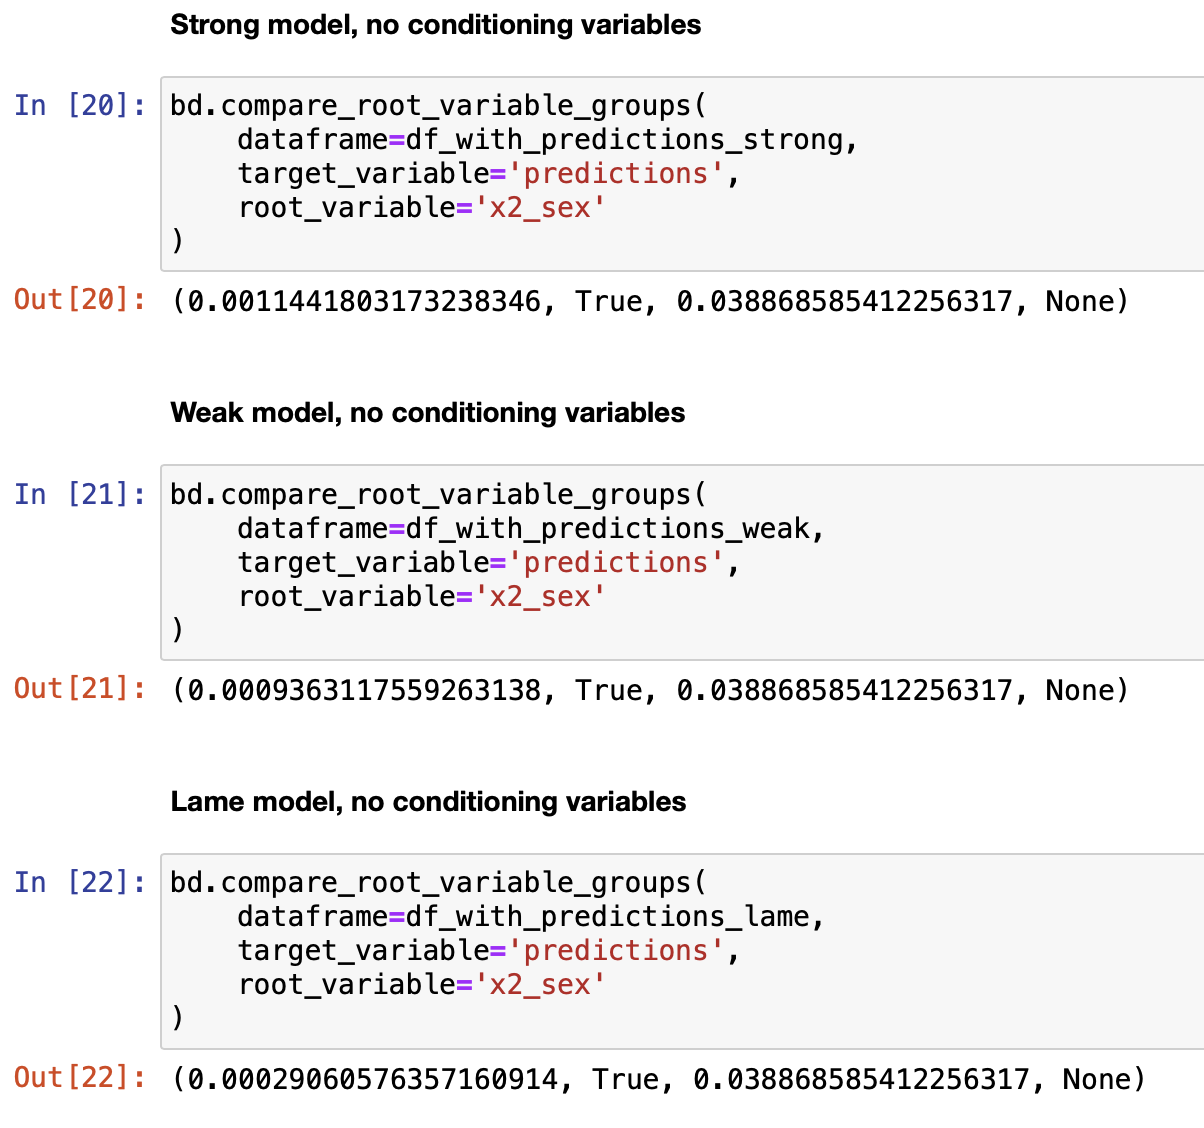
\includegraphics[width=.8\linewidth, left]{exp3.png}
  \caption{Experiment 3 results.}
  \label{fig:exp3}
\end{figure}
Figure \ref{fig:exp3} shows the results of the third experiment. Now we are interested in trying out the other distance, the JS divergence, provided by the tool for the freqs-vs-freqs analysis. As expected, the distances are of a smaller order of magnitude. Apart from this numerical outcome, the pattern is the same observed for Experiment 1. 

\subsubsection{Experiment 4: freqs-vs-freqs, JS, A1=low, root-variable=v3-education}

\begin{figure}[h!]
  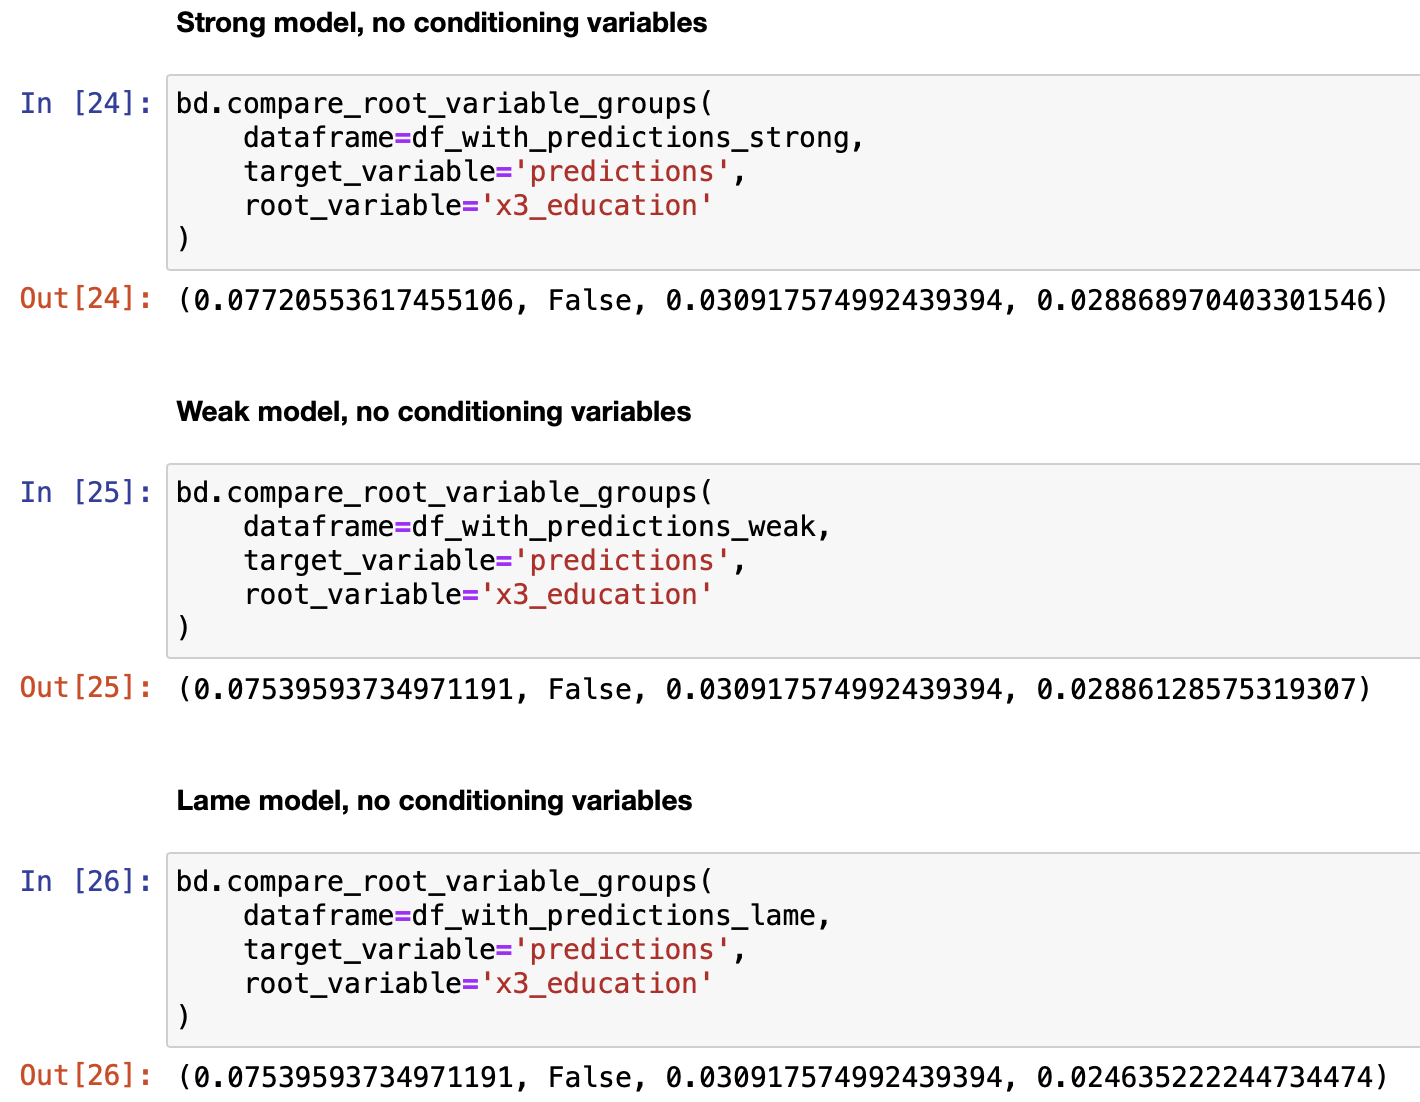
\includegraphics[width=.8\linewidth, left]{exp4.png}
  \caption{Experiment 4 results.}
  \label{fig:exp4}
\end{figure}
Figure \ref{fig:exp4} shows the results of the fourth experiment. As with Experiment 2, we observe almost identical distance values for the three models, but of a smaller order of magnitude given that we are using JS instead of TVD. 

\subsubsection{Experiment 5: freqs-vs-freqs, JS, A1=low, root-variable=x6-pay-0 (discrete)}

\begin{figure}[h!]
  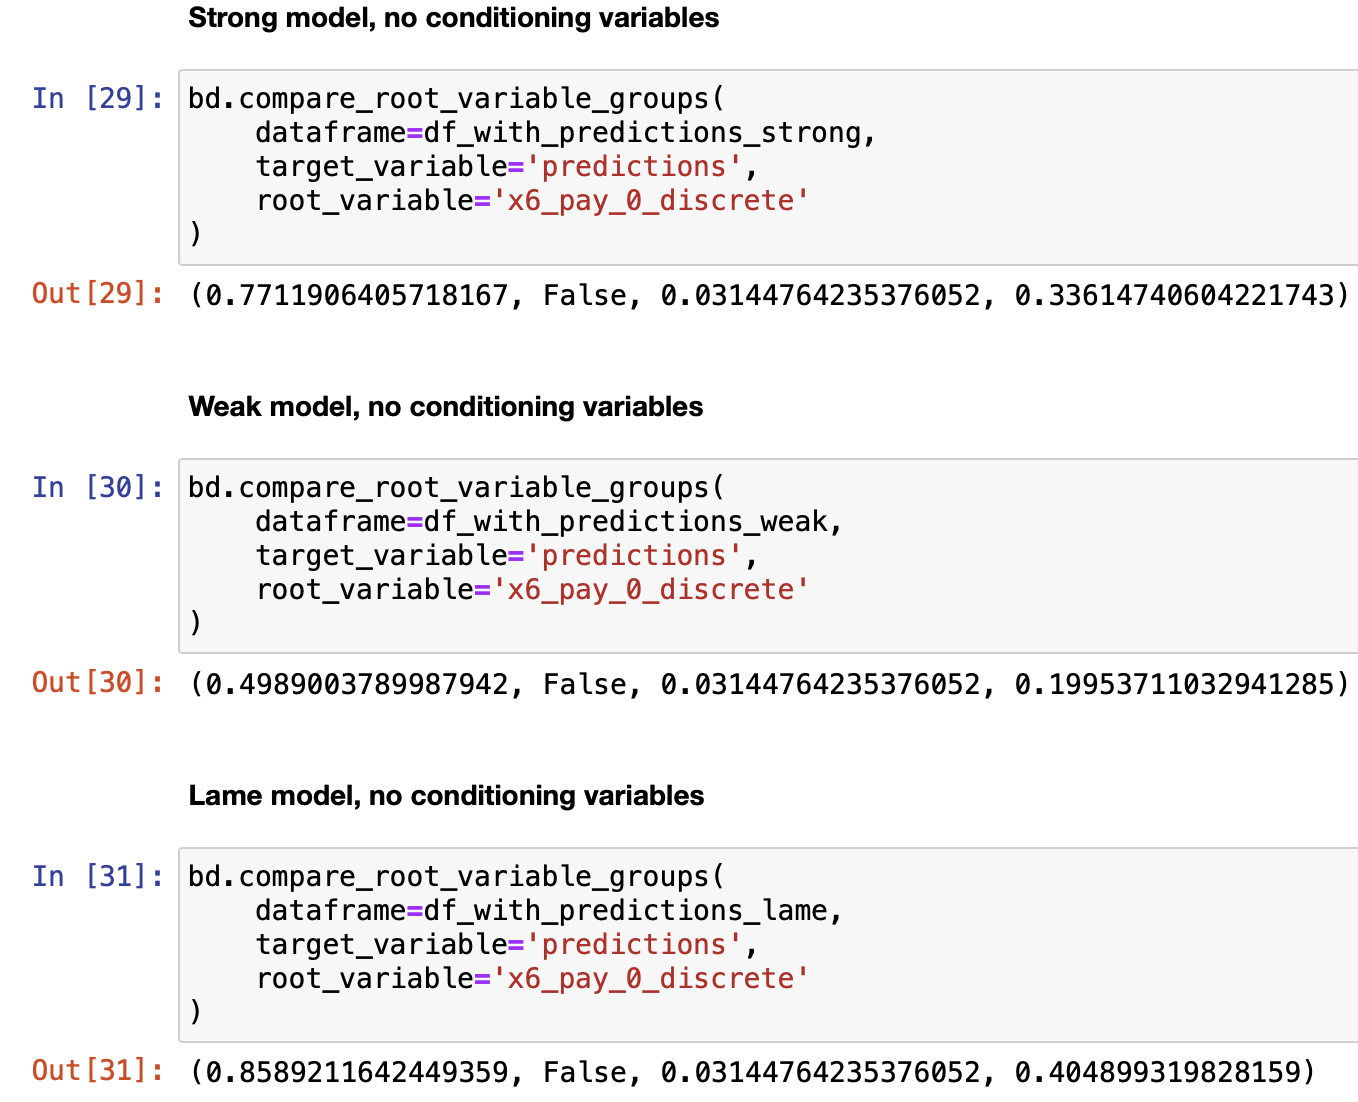
\includegraphics[width=.8\linewidth, left]{exp5.png}
  \caption{Experiment 5 results.}
  \label{fig:exp5}
\end{figure}
Figure \ref{fig:exp5} shows the results of the fifth experiment. Keeping JS as distance of choice, we wanted to verify what happens if the sensitive feature is also the single most important feature for the classifiers. In this case, we identified \texttt{x6-pay-0}, namely a categorical feature providing the strongest predictive signal. Clearly, being strongly effective in discriminating between true $0$ and $1$ labels, it produces way bigger distances than those observed in the previous experiments. As commented for \texttt{Education}, we imagine that it would not make sense to consider such a feature a sensitive one. Finally, large standard deviation values are observed, suggesting that some feature categories are more effective and important for the classifiers than others. 

\subsubsection{Experiment 6: freqs-vs-freqs, JS, A1=low, root-variable=x2-sex, conditioning-variable=x6-pay-0 (discrete)}
For brevity we don't include the numerical outcome of this and the next experiment. The reader can refer to the notebook provided with the online repository (\url{https://github.com/DLBD-Department/BRIO_x_Alkemy/notebooks}). We are now interested in testing the bias detector using a ``conditioning variable'', i.e. using a further dataset feature to compute the distances with respect to the sensitive feature for each subset of observations realized by the different conditioning variable categories. As conditioning variable we use \texttt{x6-pay-0}, the same feature we used in Experiment 5 as sensitive feature. It seems reasonable to ask whether, given the groups implied by a strong predictor, different bias profiles emerge. The aim is to find potential biases that are balanced out when the check is performed on the overall population, but which emerge when focusing on specific subgroups of individuals. In this experiment we use the JS Divergence. 

It seems clear that the computed distances can vary a lot for the different conditioning variable groups, justifying our interest in this kind of check. This behavior is stronger when the model is particularly accurate in its predictions, e.g. for the ``strong'' model results. On the other hand, the ``lame'' model produces distances equal to zero for each subgroup, given that it's not able to use \texttt{x6-pay-0} to discriminate between observations. 

\subsubsection{Experiment 7: freqs-vs-freqs, TVD, A1=low, root-variable=x2-sex, conditioning-variable=x6-pay-0 (discrete)}
In this final experiment we repeat the same setting of Experiment 6 but using TVD instead of JS. The observed pattern is identical, with the already commented distances magnitude difference due to the different distance used here. 

\section{Conclusions and Further Work}
\label{sec:conclusions}

The tool for the detection of biases in AI systems presented in this paper is meant to be the first module to be integrated into a more complex software application. The complete system will present additionally a module for the evaluation of opacity values. The system will be completed by a third module whose aim will be to take in input the output of the bias and opacity modules, to return the user with a risk evaluation associated with the use of the dataset or model under analysis. We leave the presentation of these two additional modules to future work.


% consisting of three, partly inter-dependent modules. The complete system will present two autonomous modules for the analysis of bias and opacity of AI systems---the first of which we just presented---and a module depending on these two concerning risk evaluation.

%\section{Acknowledgments}
%
%Identification of funding sources and other support, and thanks to
%individuals and groups that assisted in the research and the
%preparation of the work should be included in an acknowledgment
%section, which is placed just before the reference section in your
%document.
%
%This section has a special environment:
%\begin{lstlisting}
%\begin{acknowledgments}
%  These are different acknowledgments.
%\end{acknowledgments}
%\end{lstlisting}
%so that the information contained therein can be more easily collected
%during the article metadata extraction phase, and to ensure
%consistency in the spelling of the section heading.
%
%Authors should not prepare this section as a numbered or unnumbered
%\verb|\section|; please use the ``\verb|acknowledgments|'' environment.


%%
%% The acknowledgments section is defined using the "acknowledgments" environment
%% (and NOT an unnumbered section). This ensures the proper
%% identification of the section in the article metadata, and the
%% consistent spelling of the heading.
\begin{acknowledgments}
This research has been partially funded by the Project PRIN2020 ``BRIO - Bias, Risk and Opacity in AI'' (2020SSKZ7R) and by by the Department of Philosophy ``Piero Martinetti'' of the University of Milan under the Project ``Departments of Excellence 2023-2027'', both awarded by the Ministry of University and Research (MUR).
\end{acknowledgments}

%%
%% Define the bibliography file to be used
\bibliography{sample-ceur}

%%
%% If your work has an appendix, this is the place to put it.
\appendix

\section{Online Resources}
%The sources for the ceur-art style are available via
%\begin{itemize}
%\item \href{https://github.com/yamadharma/ceurart}{GitHub},
%% \item \href{https://www.overleaf.com/project/5e76702c4acae70001d3bc87}{Overleaf},
%\item
%  \href{https://www.overleaf.com/latex/templates/template-for-submissions-to-ceur-workshop-proceedings-ceur-ws-dot-org/pkfscdkgkhcq}{Overleaf
%    template}.
%\end{itemize}

The sources for the tool are available via
\begin{itemize}
\item \href{https://github.com/DLBD-Department/BRIO_x_Alkemy}{GitHub},
\end{itemize}

\end{document}

%%
%% End of file
